\documentclass[12pt]{article}
\usepackage[a4paper,margin=1in]{geometry}
\usepackage{amsmath,amssymb}
\usepackage{graphicx}
\usepackage{siunitx}
\sisetup{per-mode=symbol}
\usepackage{gvv}

\title{4.13.84}
\author{ai25btech11015 -- M Sai Rithik}
\date{}

\begin{document}
\maketitle

\section*{Question}
Find the value of \(k\) such that the line
\[
\frac{x-4}{1}=\frac{y-2}{1}=\frac{z-k}{2}
\]
lies in the plane
\[
2x-4y+z=7.
\]

\section*{Solution}

Write the line in the standard parametric matrix form using a general position vector $\Vec{p}$ and direction vector $\Vec{v}$:
\begin{equation}
\Vec{r}(t) \;=\; \myvec{x\\y\\z} \;=\; \Vec{p} + t\,\Vec{v},
\label{eq:rt}
\end{equation}
where $\Vec{p}$ is any point on the line and $\Vec{v}$ is the direction vector.

The plane can be written using its normal vector $\Vec{n}$ as a dot-product condition:
\begin{equation}
\Vec{n}^{T}\,\Vec{r} = 7.
\label{eq:plane}
\end{equation}

Substitute \eqref{eq:rt} into \eqref{eq:plane} and use linearity:
\begin{equation}
\Vec{n}^{T}(\Vec{p} + t\Vec{v}) = 7.
\label{eq:lin}
\end{equation}

Distribute the transpose-dot product:
\begin{equation}
\Vec{n}^{T}\Vec{p} \;+\; t\,\Vec{n}^{T}\Vec{v} \;=\; 7.
\label{eq:separate}
\end{equation}

For the entire line to lie in the plane the identity \eqref{eq:separate} must hold for all real \(t\).  
Hence the coefficient of \(t\) must be zero and the constant term must equal \(7\).  Thus we obtain the two matrix equations:
\begin{align}
\Vec{n}^{T}\Vec{v} &= 0, \label{eq:tvanish} \\
\Vec{n}^{T}\Vec{p} &= 7. \label{eq:constcond}
\end{align}

Now substitute the specific normal, position and direction vectors from the problem:
\begin{align}
\Vec{n} &= \myvec{2\\-4\\1}, \label{eq:n} \\
\Vec{p} &= \myvec{4\\2\\k}, \label{eq:p} \\
\Vec{v} &= \myvec{1\\1\\2}. \label{eq:v}
\end{align}

Evaluate the \(t\)-coefficient condition \eqref{eq:tvanish} by matrix multiplication:
\begin{equation}
\Vec{n}^{T}\Vec{v}
= \begin{bmatrix}2 & -4 & 1\end{bmatrix}
\myvec{1\\1\\2}
= 2\cdot 1 + (-4)\cdot 1 + 1\cdot 2
= 0.
\label{eq:tvanishcalc}
\end{equation}
So \eqref{eq:tvanish} is satisfied (no restriction on \(k\) from this equation).

Evaluate the constant condition \eqref{eq:constcond}:
\begin{equation}
\Vec{n}^{T}\Vec{p}
= \begin{bmatrix}2 & -4 & 1\end{bmatrix}
\myvec{4\\2\\k}
= 2\cdot 4 + (-4)\cdot 2 + 1\cdot k
= k.
\label{eq:constcalc}
\end{equation}

Set \eqref{eq:constcalc} equal to \(7\) and solve for \(k\):
\begin{equation}
k = 7.
\label{eq:kfinal}
\end{equation}

\section*{Answer}
\begin{equation}
\boxed{k = 7}
\end{equation}

\begin{figure}[h!]
    \centering
    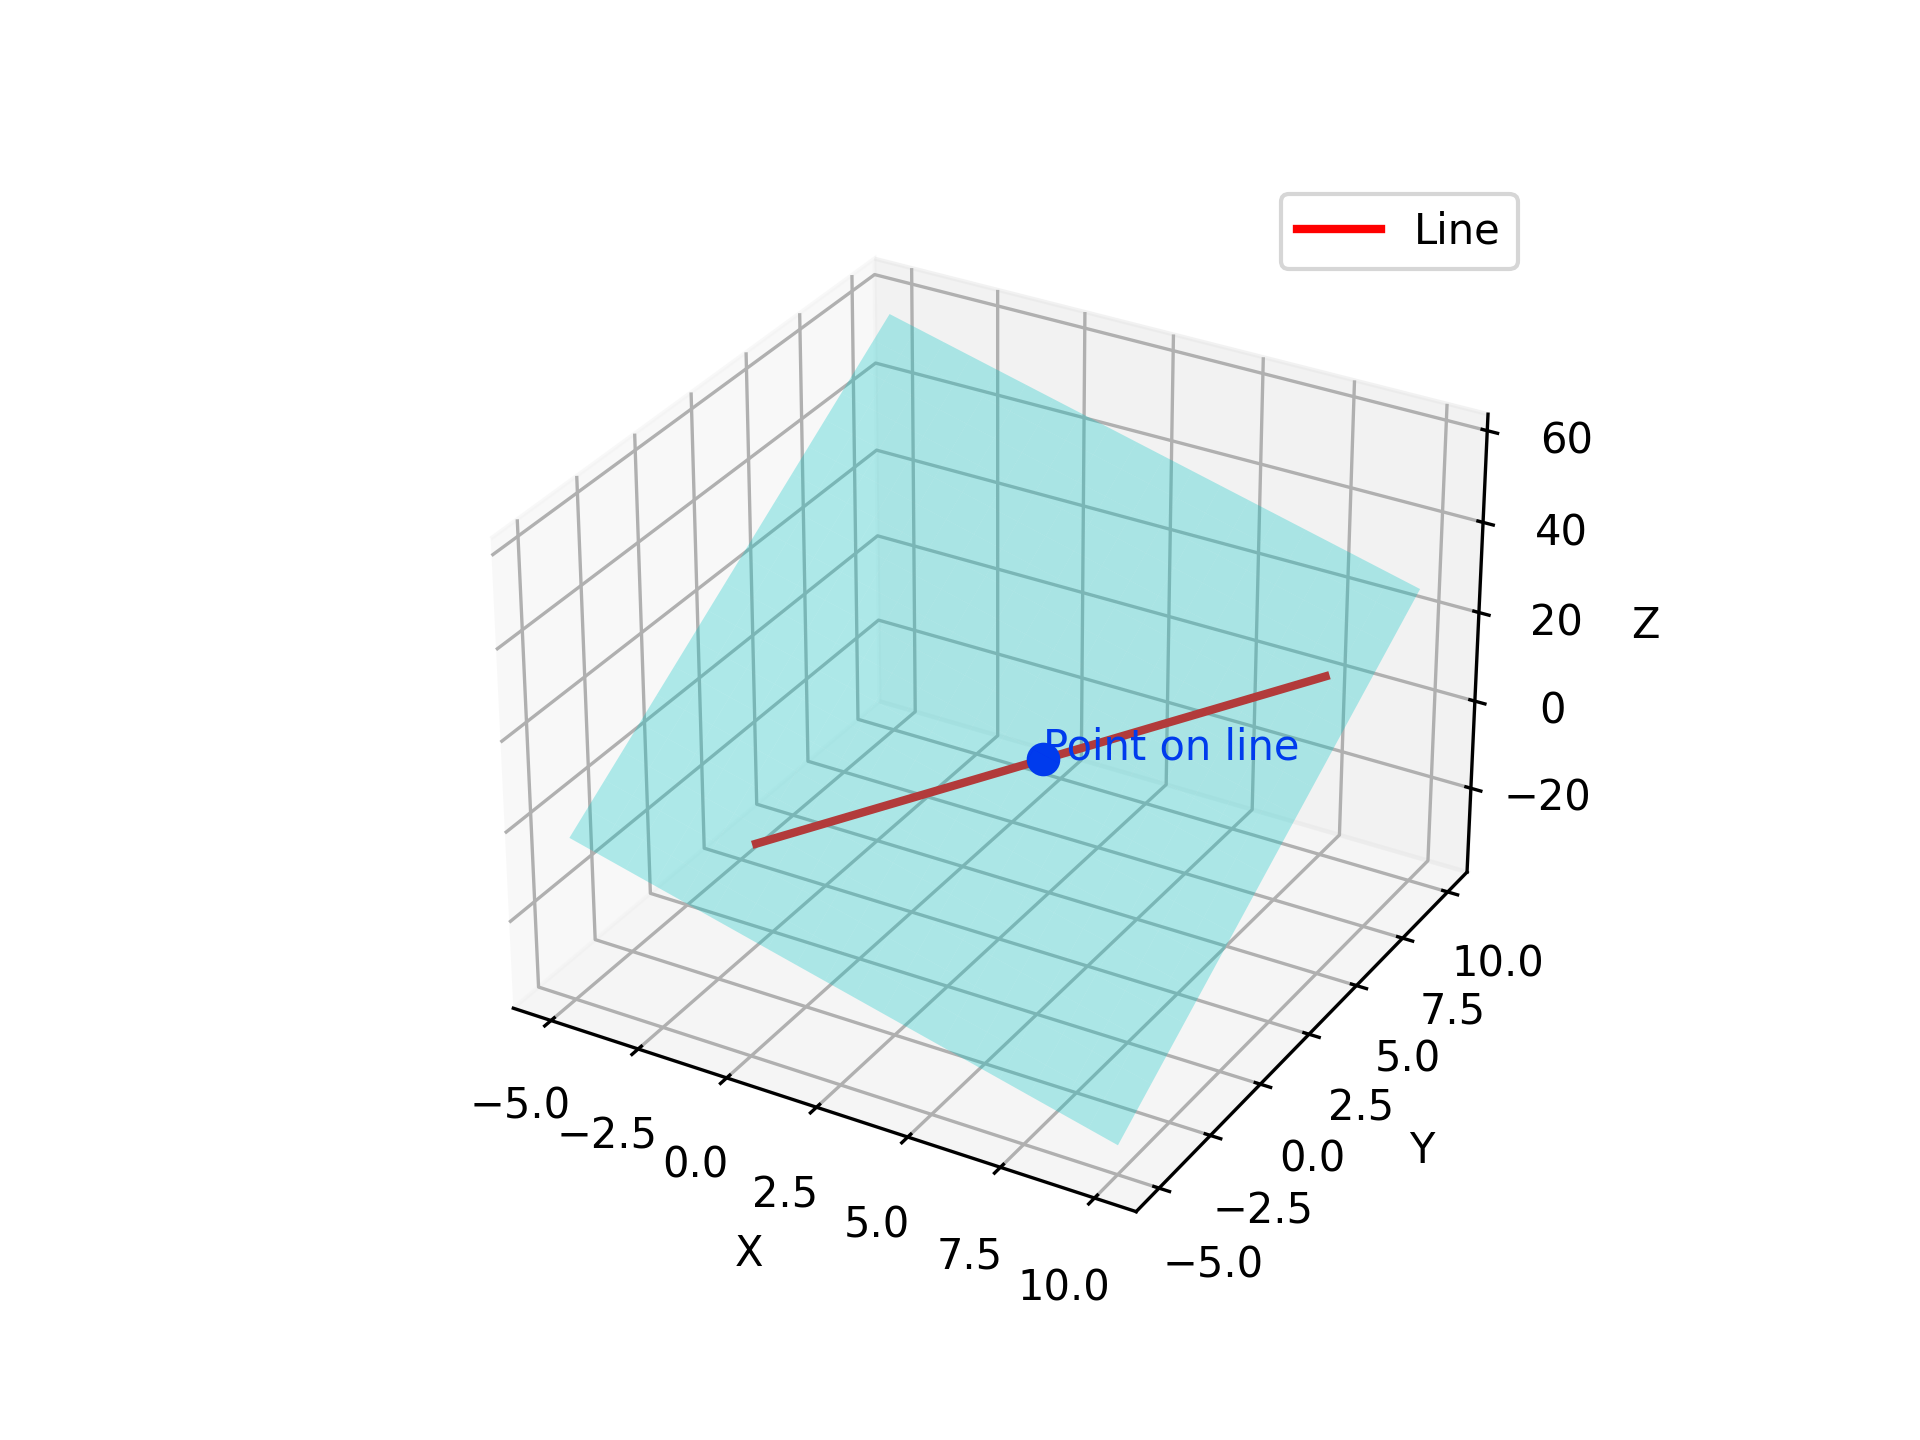
\includegraphics[width=0.65\linewidth]{figs/fig.png}
    \caption{(Sketch: plane through $A,B,C$).}
\end{figure}
\end{document}
